\section*{Section C}
\label{sec:Section C}
\FloatBarrier % Now figures cannot float above section title

In this section, finite element analysis (ANSYS) is performed on the components.

\subsection*{Analysis}

ANSYS analysis results are shown in Figure \ref{f2}.

\begin{figure}[htbp]
    \centering
    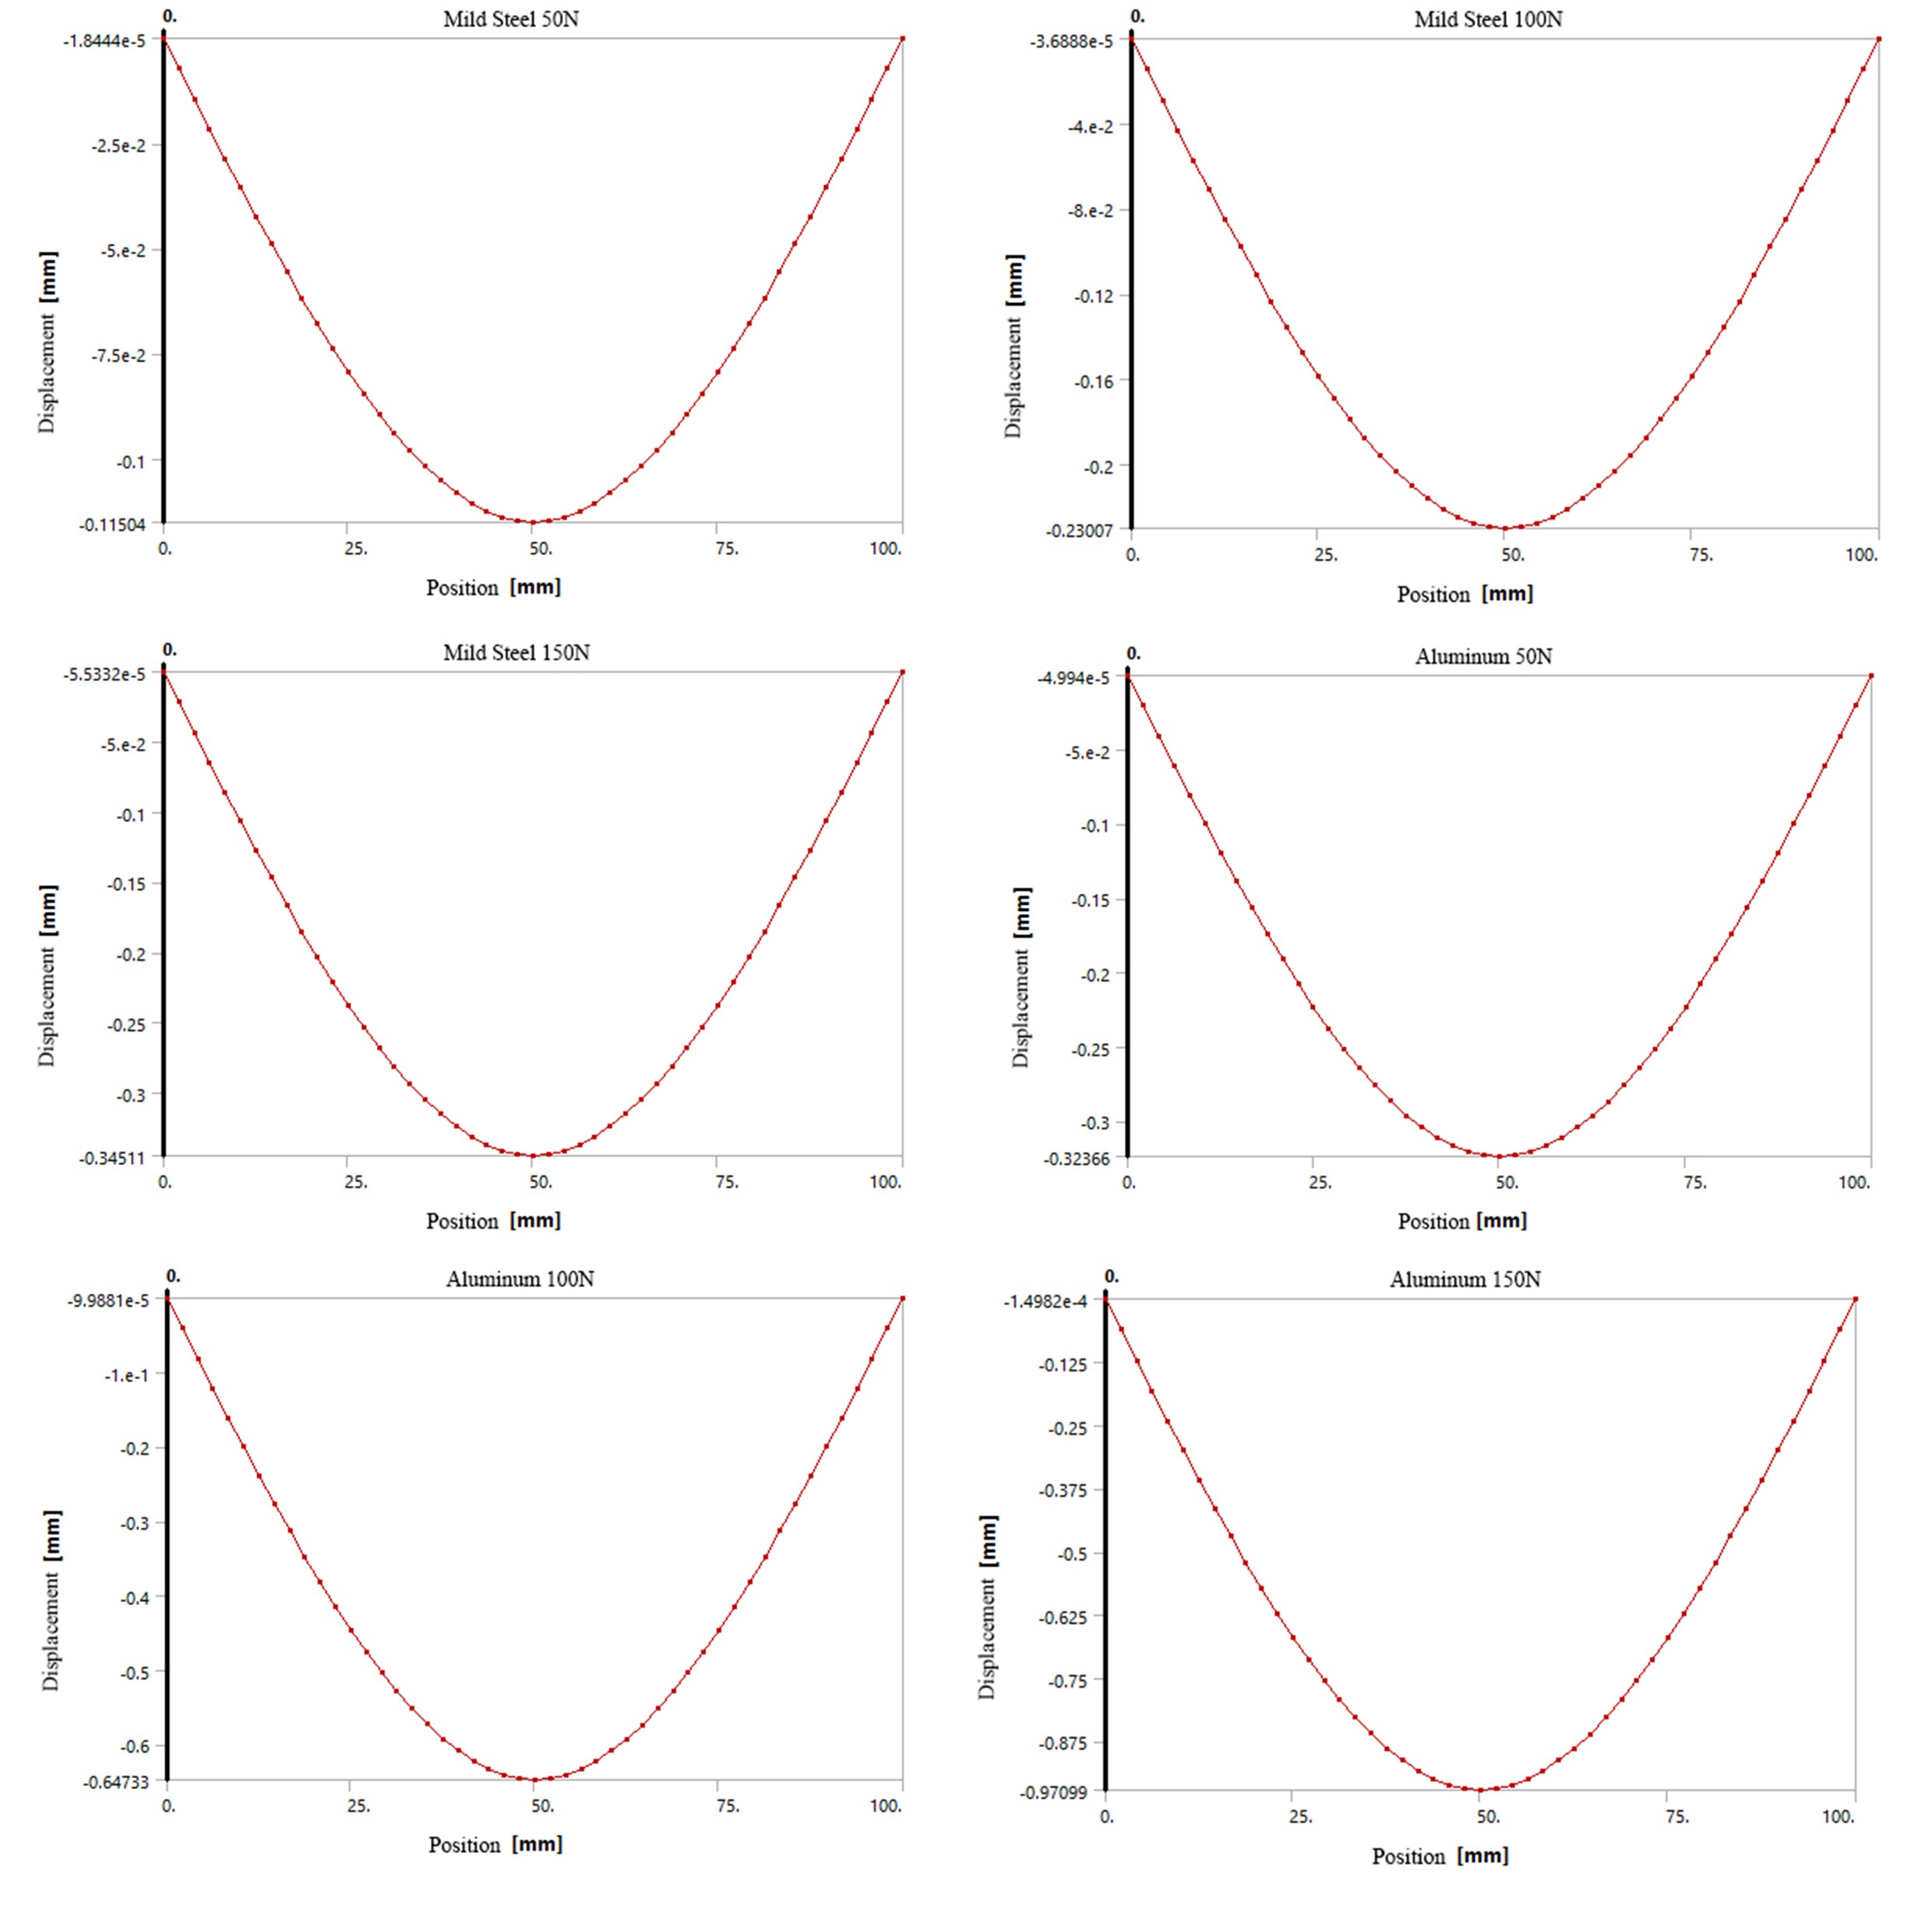
\includegraphics[width=18cm,height=20cm]{./fig/mix2.jpg}
    \caption{Figure of ANSYS analysis}
    \label{f2}
\end{figure}


The finite element analysis in Figure \ref{f2} gives the deformation-position 
curves for different materials under different forces, 
where the maximum deformation of the component can be easily determined.

The data are shown in Table \ref{t4}.

\begin{minipage}[htbp]{\textwidth}
    \makeatletter\def\@captype{table}
    \centering
    \scalebox{1.1}{
    \begin{tabular}{lll} 
        \hline
        Bending Displacement  & Mild Steel    & Aluminium     \\ \hline
        $\delta_{FE\_{1}}(P=50N)$ & 0.1150    & 0.3237    \\
        $\delta_{FE\_{2}}(P=100N)$ & 0.2300    & 0.6473  \\
        $\delta_{FE\_{3}}(P=150N)$ & 0.3451    & 0.9710  \\ \hline          
    \end{tabular}} 
    
    (Unit: mm)
    \caption{FEA results - maximum deformation}
    \label{t4} 
\end{minipage}



\subsection*{Summary}
By using ANSYS analysis, deformation-displacement diagrams were obtained 
for two materials under three different forces, revealing that the maximum 
deformation exists at the midpoint of the element (the point where the forces are applied).
